\documentclass{article}
\usepackage[affil-it]{authblk}
\usepackage{xspace,xcolor}
\usepackage{graphics}
\usepackage[screen,nopanel,white]{pdfscreen}
\hypersetup{pdftoolbar=true}
\usepackage[display]{texpower}
%%%

%%% for abbreviations, or acronyms
\usepackage[acronym, nopostdot]{glossaries}  % automake
\renewcommand*{\glstextformat}[1]{\textcolor{blue}{#1}}	% removal default blue in abbreviation
\usepackage{glossary-inline}
%\setacronymstyle{long-short}
%\renewcommand*{\glossarysection}[2][]{} 
%\renewcommand*{\glossarysection}[2][]{\textbf{#1}: }
% for abbreviations environment
%\newcommand{\abbrlabel}[1]{\makebox[3cm][l]{\textbf{#1}\ \dotfill}}
\newenvironment{abbreviation}

%\section{abbreviation}
%%%%%%%%%%%%% Define abbreviation
\makeglossaries %https://tex.stackexchange.com/questions/110095/list-of-acronyms-is-not-displayed

\newacronym{ncbi}{NCBI}{National Center for Biotechnology Information}
\newacronym{degs}{DEGs}{differentially expressed genes}

\newacronym{ihc}{IHC}{immunohistochemistry}
\newacronym{fdr}{FDR}{false discovery rate}

\newacronym{hpa}{HPA}{the Human Protein Atlas}
\newacronym{hnscc}{HNSCC}{head and neck squamous cell carcinoma}
\newacronym{tcga}{TCGA}{the Cancer Genome Atlas}
\newacronym{tcpa}{TCPA}{the Cancer Proteome Atlas}
\newacronym{rna}{RNA}{ribonucleic acid}
\newacronym{rnaseq}{RNA-Seq}{RNA sequencing}
\newacronym{lncrna}{lncRNA}{long non-coding RNA}
%\newacronym{km}{KM}{Kaplan--Meier}
\newacronym{rppa}{RPPAs}{reverse-phase protein arrays}
\newacronym{rpma}{RPMA}{reverse-phase protein lysate microarray}

\newacronym{mmp}{MMP}{matrix metalloproteinase}
 %DKK1, CAMK2N1, STC2, PGK1, SURF4, USP10, NDFIP1, FOXA2, STIP1, and DKC1
 %ZNF557, ZNF266, IL19, MYO1H, FCGBP, LOC148709, EVPLL, PNMA5, KIAA1683, and NPB

\newacronym{DKK1}{DKK1}{dickkopf WNT signaling pathway inhibitor 1} 
\newacronym{CAMK2N1}{CAMK2N1}{calcium/calmodulin dependent protein kinase II inhibitor 1} 
\newacronym{CALML5}{CALML5}{calmodulin like 5}

\newacronym{STC2}{STC2}{stanniocalcin 2} 
\newacronym{PGK1}{PGK1}{phosphoglycerate kinase 1} 
\newacronym{SURF4}{SURF4}{surfeit 4} 
\newacronym{USP10}{USP10}{ubiquitin specific peptidase 10} 
\newacronym{NEDD4}{NEDD4}{neural precursor cell expressed, developmentally down-regulated 4}
\newacronym{NDFIP1}{NDFIP1}{NEDD4 family interacting protein 1} 
\newacronym{FOXA2}{FOXA2}{forkhead box A2} 
\newacronym{STIP1}{STIP1}{stress-induced-phosphoprotein 1} 
\newacronym{DKC1}{DKC1}{dyskeratosis congenita 1, dyskerin} 

\newacronym{ZNF557}{ZNF557}{zinc finger protein 557} 
\newacronym{ZNF266}{ZNF266}{zinc finger protein 266} 
\newacronym{IL19}{IL19}{interleukin 19} 
\newacronym{MYO1H}{MYO1H}{myosin 1H} 
\newacronym{FCGBP}{FCGBP}{Fc fragment of IgG binding protein} 
\newacronym{LOC148709}{LOC148709}{LncRNA LOC148709} 
\newacronym{EVPLL}{EVPLL}{envoplakin-like protein} 
\newacronym{PNMA5}{PNMA5}{paraneoplastic antigen like 5} 
%\newacronym{KIAA1683}{KIAA1683}{IQCN, IQ Motif Containing N} 
\newacronym{IQCN}{IQCN}{IQ motif containing N} % previous name KIAA1683
% "IQ'' refers to the first two amino acids of the motif: isoleucine (commonly) and glutamine (invariably)
\newacronym{NPB}{NPB}{neuropeptide B} 

 \newacronym{rt}{RT}{radiation therapy}
 \newacronym{nccn}{NCCN}{National Comprehensive Cancer Network}
 \newacronym{hif}{HIF}{hypoxia-inducible factor}
 \newacronym{egfr}{EGFR}{epidermal growth factor receptor}
 \newacronym{ras}{RAS}{rat sarcoma}
 \newacronym{hras}{HRAS}{Harvey rat sarcoma viral oncoprotein}
 \newacronym{erk}{ERK}{extracellular signal-regulated kinases}
 \newacronym{us}{US}{United States}
 \newacronym{fda}{FDA}{Food and Drug Administration}
 \newacronym{tpf}{Tax-PF}{docetaxel, cisplatin, and 5-fluorouracil}
 \newacronym{tki}{TKI}{tyrosine kinase inhibitor}
 \newacronym{her}{HER}{human epidermal growth factor receptor}
 \newacronym{ici}{ICI}{immune-checkpoint inhibitor}
 \newacronym{ctla4}{CTLA-4}{cytotoxic T lymphocyte antigen 4}
 \newacronym{pd1}{PD-1}{programmed death 1}
 \newacronym{pdl1}{PD-L1}{programmed death ligand 1}
 \newacronym{tim3}{TIM-3}{T-cell immunoglobulin mucin protein 3}
 \newacronym{lag3}{LAG-3}{lymphocyte activation gene 3}
 \newacronym{ifng}{IFN-$\gamma$}{interferon gamma}
 \newacronym{tigit}{TIGIT}{T cell immunoglobin and immunoreceptor tyrosine-based inhibitory motif}
 \newacronym{gitr}{GITR}{glucocorticoid-induced tumor necrosis factor receptor}
 \newacronym{vista}{VISTA}{V-domain Ig suppressor of T-cell activation}
 \newacronym{tmsb4x}{TMSB4X}{thymosin beta-4 X-linked}
 \newacronym{emt}{EMT}{epithelial-mesenchymal-transition}
 \newacronym{gdc}{GDC}{Genomic Data Commons}
 \newacronym{nci}{NCI}{the National Cancer Institute}
 \newacronym{gdac}{GDAC}{genome data analysis center}
 \newacronym{rest}{REST}{Representational State Transfer} 
 \newacronym{api}{API}{application programmable interface}
\newacronym{grch38}{GRCh38}{Genome Reference Consortium Homo sapiens genome assembly 38}
\newacronym{fpkm}{FPKM}{Fragments per kilobase per million reads mapped}
\newacronym{rsem}{RSEM}{RNA-Seq by Expectation-Maximization}
\newacronym{slca}{SLC35E2A}{solute carrier family 35 member E2A}
\newacronym{slcb}{SLC35E2B}{solute carrier family 35 member E2B}
\newacronym{cde}{CDE}{Common Data Element}
\newacronym{id}{ID}{identification}
\newacronym{ajcc}{AJCC}{the American Joint Committee on Cancer}
\newacronym{uicc}{UICC}{he Union for International Cancer Control}
\newacronym{tnm}{TNM}{the tumor size (T), cervical lymph node metastases (N), and distal metastasis status (M)}
\newacronym{ci95}{95\% CI}{95\% confidence interval}
\newacronym{os}{OS}{overall survival}
\newacronym{hr}{HR}{hazard ratio}
\newacronym{hpv}{HPV}{human papillomavirus}
\newacronym{ene}{ENE}{extra-nodal extension}
\newacronym{lvsi}{LVSI}{lymph-vascular space invasion}
\newacronym{pni}{PNI}{perineural invasion}
\newacronym{doi}{DOI}{depth of invasion}
\newacronym{lnd}{LND}{lymph node density}
\newacronym{wpoi5}{WPOI-5}{worst pattern of invasion score 5}
\newacronym{glut4}{GLUT4}{glucose transporter 4}
\newacronym{slc2a4}{SLC2A4}{solute carrier family 2 member A4}
\newacronym{trim24}{TRIM24}{tripartite motif-containing 24}
\newacronym{til}{TIL}{tumor-infiltrating lymphocytes}
\newacronym{tmb}{TMB}{tumor mutational burden}

%%%
\margins{0.25in}{0.25in}{0.25in}{0.25in}
\screensize{297mm}{210mm}% 4.5in by 8in for widescreen
\backgroundcolor{white} %blue
\color{black} % text color

\author[1]{Chi, Li-Hsing (Tex)} %, D.D.S., Ph.D. candidate}
\author[1]{Wu, TH Alex}
\author[2]{Hsiao, Michael}
\author[1]{Li, Yu-Chuan (Jack)}
\affil[1]{The Ph.D. Program for Translational Medicine, College of Medical Science and Technology, Taipei Medical University and Academia Sinica}
\affil[2]{Genomics Research Center, Academia Sinica}
\title{A Transcriptomic Analysis of Head and Neck Squamous Cell Carcinomas for Prognostic Indications} % pvalueTex

\begin{document}
\maketitle

\section{Abstract}
\textbf{Background:} Survival analysis of \acrfull{tcga} dataset is a well-known method for discovering gene expression-based prognostic biomarkers of \acrfull{hnscc}.
A cutoff point is usually used in survival analysis for patient dichotomization when using continuous gene expression values. There is some optimization software for cutoff determination. However, the software's predetermined cutoffs are usually set at the medians or quantiles of gene expression values. There are also few clinicopathological features available in pre-processed datasets.\\
\textbf{Method:} We applied an in-house workflow, including data retrieving and pre-processing, feature selection, sliding-window cutoff selection, Kaplan--Meier survival analysis, and Cox proportional hazard modeling for biomarker discovery.
In our approach for the TCGA HNSCC cohort, we scanned human protein-coding genes to find optimal cutoff values.\\
\textbf{Result:} After adjustments with confounders, clinical tumor stage and surgical margin involvement were found to be independent risk factors for prognosis. According to the results tables that show hazard ratios with Bonferroni-adjusted \textit{p}~values under the optimal cutoff, three biomarker candidates, \acrshort{CAMK2N1}, \acrshort{CALML5}, and \acrshort{FCGBP}, are significantly associated with overall survival. We validated this discovery by using the another independent HNSCC dataset (GSE65858).\\
\textbf{Conclusion:} Thus, we suggest that transcriptomic analysis could help with biomarker discovery. Moreover, the robustness of the biomarkers we identified should be ensured through several additional tests with independent datasets.



\textbf{Keywords:}
head and neck squamous cell carcinoma (HNSCC);
the Cancer Genome Atlas (TCGA); transcriptomic analysis; survival analysis; optimal cutoff; effect size; \acrfull{CAMK2N1}; \acrfull{CALML5}; \acrfull{FCGBP}; mindfulness meditation

\vspace{1cm}
\includegraphics[width=15cm]{graphic_abstract_pvalueTex.jpeg}
\clearpage

\begin{figure}[ht]
%\floatbox[{\capbeside\thisfloatsetup{capbesideposition={right,center},capbesidewidth=.35\linewidth,capbesidesep=quad}}]{figure}[\FBwidth]
%\centering
%\widefigure, keepaspectratio
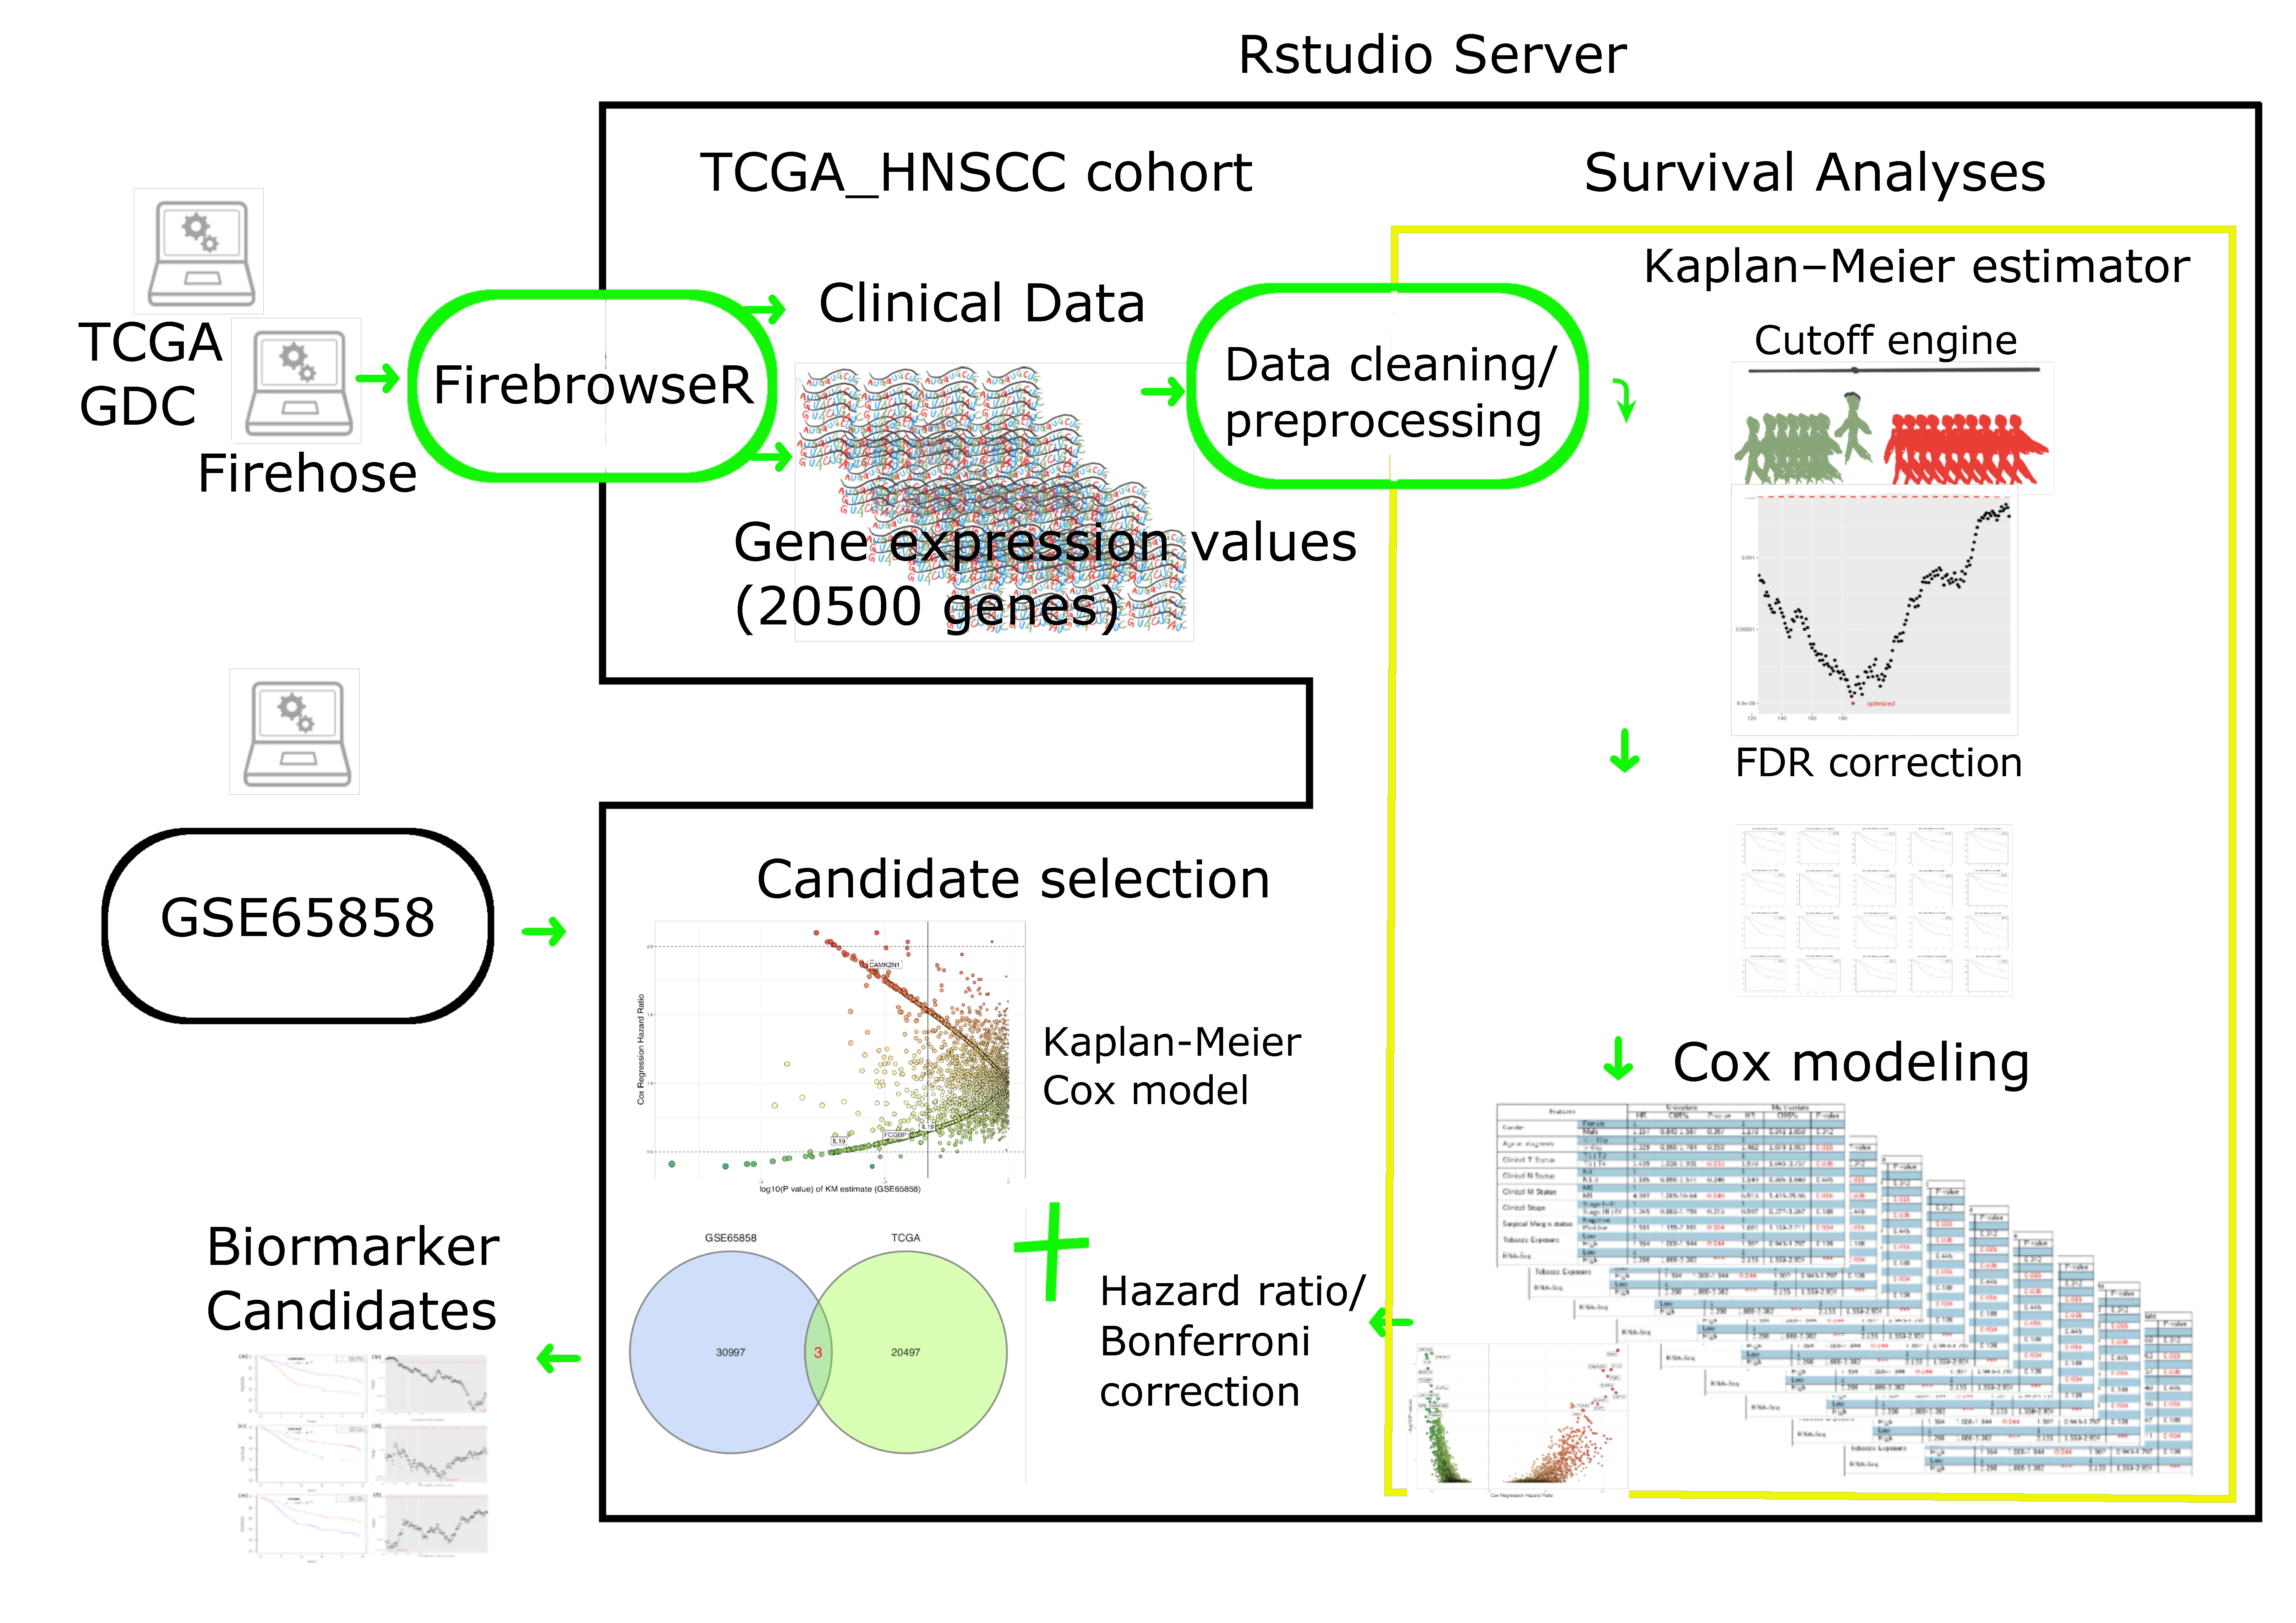
\includegraphics[width=7cm]{Figure_1_manuscript_workflow.pdf} % .PDF is better than .png
%, height=8cm
%\caption % , step 1 (\textcolor{blue}{blue line}: main procedure) and step 2 (\textcolor{orange}{orange line}: analysis export).
%Step 3 (purple line: dealing with surgical margin).
%\sidecaptionvpos{c}
\caption{\hl{A workflow of \acrshort{hnscc} biomarker discovery.\\
The workflow includes data retrieval from the TCGA GDC data portal, data processing with merging and cleaning, and then performing the survival analyses (within \textcolor{yellow}{yellow} square).} The Cutoff engine (in R script: cutofFinder\_func.HNSCC.R, a serial cutoff for grouping patients with \textcolor{asparagus}{low} or \textcolor{red}{high} expression of a specific gene, to yield a collection of \protect\textit{P} values; please see Materials and Methods section for details) might calculate all possible Kaplan--Meier \protect\textit{P} values (corrected by \acrlong{fdr}, FDR, method) to find the optimal cutoff value of gene expression for subsequent Cox modeling. The candidate selection performs (1) dissecting and selection of candidate genes with further Bonferroni adjusted \protect\textit{P} values and the hazard ratios of a Cox model, based on the results from the survival analyses; (2) survival analyses of the other HNSCC dataset (GSE65858) using Kaplan--Meier estimates (with FDR corrections) and Cox modeling.\\ The biomarker candidates were consensus results of TCGA and GSE65858. (HNSCC: head and neck squamous cell carcinoma; TCGA: the Cancer Genome Atlas; RNA-Seq: RNA sequencing; GDC: Genomic Data Commons.)}  % end of caption

% Description:1) FDR correction of Kaplan--Meier \protect\textit{P} values during Cutoff finding; and 2) Bonferroni correction of Kaplan--Meier \protect\textit{P} values after Cox modeling for candidate selection.

%\end{minipage}
\end{figure}

\clearpage

\section{Results}


\section{sec2}
\subsection{sec1.1}

See the data in \ref{fig:1}.

\section*{Figures}
\begin{figure}
    \includegraphics[scale = 0.5]{example-image}
    \caption{No caption, No figure number, No label}
    \label{fig:1}
\end{figure}
\end{document}